\FloatBarrier
\section{Workload characterisation}\label{sec:workload}

\subsection{Governing equations and discretisation}
A hydrostatic primitive-equation core solves, in flux form,
\begin{align}
\frac{\partial \rho}{\partial t} + \nabla\cdot(\rho\mathbf{u}) &= 0,\\
\frac{\partial (\rho\mathbf{u})}{\partial t} + \nabla\cdot(\rho\mathbf{u}\otimes\mathbf{u})
  &= -\nabla p - \rho f\,\mathbf{k}\times\mathbf{u} + \rho\mathbf{g} + \mathbf{F}_{\mathrm{diff}},\\
\frac{\partial (\rho\theta)}{\partial t} + \nabla\cdot(\rho\theta\mathbf{u}) &= S_{\theta},\\
\frac{\partial (\rho q_x)}{\partial t} + \nabla\cdot(\rho q_x\mathbf{u}) &= S_{x},
  \qquad x \in \{\text{vapour, cloud, rain, ice, snow, graupel}\},
\end{align}
plus a pressure equation and a set of physical parameterisations for radiation, turbulence,
convection, microphysics and the surface. The discretisation is a 3D grid with 24 prognostic
variables; advection is semi-Lagrangian with 8-point interpolation in the horizontal and
Lagrangian vertical remapping, diffusion is biharmonic, and the physics package is evaluated
column-by-column.

The benchmark used throughout is defined in Table~\ref{tab:bench} and is deliberately modest: it
is a 3 km regional domain, 256$\times$256$\times$64 cells, 64 members, 24 variables, 4,320 time
steps of 20 s. The 25.8 GB state fits in the card's 48 GB of HBM, which makes a single-card
comparison meaningful. Full global ensembles would be distributed across many cards; the
scale-out question is discussed in Section~\ref{sec:deployment} and is outside the model.

\begin{table}[t]
\centering\small
\caption{Reference workload W1. The operation count includes dynamics and the bulk physics package;
radiation is amortised over eight steps. Chemistry beyond passive tracers is not included.}
\label{tab:bench}
\begin{tabular}{@{}llr@{}}
\toprule
Parameter & Value & Total\\
\midrule
Grid (x, y, z) & 256 $\times$ 256 $\times$ 64 & 4.19 M cells\\
Prognostic variables & 24 & \\
Ensemble members & 64 & \\
Time step / forecast length & 20 s / 24 h & 4,320 steps\\
Flops per cell per member per step & 4,540 & 5.26 PFLOP per forecast\\
SFU operations per cell & 76 & 2.0 $\times 10^{10}$ per step\\
State size (fp32) & 96 B per cell & 25.8 GB\\
HBM traffic per step & 51.5 GB & 222 TB per forecast\\
\bottomrule
\end{tabular}
\end{table}

\subsection{Kernel taxonomy and arithmetic intensity}
The ten kernels of the model are listed in Table~\ref{tab:kernels}. Three observations drive the
architecture.

\begin{table}[t]
\centering\small
\caption{Kernel composition of the reference step. Efficiency is the sustained issue efficiency of
the AVT pipeline model (Section~\ref{sec:micro}); the last two columns are shares of the chip
totals.}
\label{tab:kernels}
\begin{tabular}{@{}lrrrrr@{}}
\toprule
Kernel & GFLOP/step & SRAM B/cell & Efficiency & Cycle share & Energy share\\
\midrule
Semi-Lagrangian advection & 2,818.6 & 200 & 79.1\% & 43.3\% & 43.4\%\\
Biharmonic diffusion & 590.6 & 200 & 79.1\% & 9.1\% & 9.1\%\\
Pressure gradient + Coriolis & 697.9 & 100 & 79.1\% & 10.7\% & 10.7\%\\
Bulk microphysics (28 SFU) & 1,664.3 & 100 & 72.3\% & 22.9\% & 22.8\%\\
PBL turbulence (6 SFU) & 1,073.7 & 80 & 76.2\% & 14.1\% & 14.0\%\\
Convection (12 SFU) & 1,395.8 & 64 & 72.9\% & 19.1\% & 19.1\%\\
Radiation, 1/8 amortised (26 SFU) & 2,039.9 & 64 & 69.8\% & 29.1\% & 29.0\%\\
Surface / land (4 SFU) & 617.2 & 48 & 77.6\% & 7.9\% & 7.8\%\\
Tracer chemistry & 966.2 & 64 & 84.8\% & 11.3\% & 11.2\%\\
Conservation audit & 322.1 & 100 & 82.9\% & 3.9\% & 3.9\%\\
\bottomrule
\end{tabular}
\end{table}

\textbf{The step is dominated by advection and radiation.} Together they account for 55\% of the
dynamic instruction count. Advection is stencil-heavy and latency-tolerant; radiation is
SFU-heavy (exponentials, logarithms, optical-depth table lookups) and latency-sensitive. A machine
that only optimises FMA throughput would be badly balanced.

\textbf{The working set is small, the stream is large.} A tile of 910 cells, 24 variables and three
time levels fits in 256 KB. The full state does not fit anywhere on chip: 25.8 GB must cross the
HBM boundary once per step, 51.5 GB of read-plus-write, and that traffic costs 0.82 J of the
1.26 J step budget.

\textbf{Physics is SFU-bound at the margin.} 76 special-function operations per cell at a
quarter-rate SFU is 304 issue slots against 2,270 FMA slots --- 13\% of the compute time, but a
larger share of the dependent stalls because the SFU latency is exposed. The tile model reflects
this in the lower efficiency of the microphysics and radiation kernels.

\subsection{Ensembles and data assimilation}
An ensemble forecast is $K$ independent integrations of the same model. A cycled analysis adds an
ensemble Kalman filter between forecast segments: the background covariance is estimated from the
$K$ members, the gain is applied to perturbed observations, and the analysis is inflated to
prevent filter divergence. In the reference day the forecast contributes 5.26 PFLOP and four
analyses contribute a further $4\times0.25\times5.26 = 5.26$ PFLOP-equivalent, i.e. the analysis
is half of the daily arithmetic.

The two phases have opposite hardware personalities. The forecast is stencil-dominated,
memory-heavy and latency-tolerant; the analysis is dense linear algebra, compute-heavy and
latency-sensitive. \ac{1} is designed for the first and is merely competent at the second
(Section~\ref{sec:results} quantifies both, including the case where the GPU wins).

\subsection{What the hardware must provide}
Table~\ref{tab:req} translates the workload into requirements. The right-hand column is what a
general-purpose GPU provides today; the gap is the design space.

\begin{table}[t]
\centering\small
\caption{Workload requirements versus a general-purpose GPU. ``GPU'' refers to the H100 SXM5
baseline used in Section~\ref{sec:results}.}
\label{tab:req}
\begin{tabularx}{\linewidth}{@{}lXl@{}}
\toprule
Requirement & Why & GPU today\\
\midrule
High stencil efficiency & 23.6 flop/byte at HBM, 20--30\% of peak is typical & 22--50\%\\
Ensemble parallelism & 64 independent trajectories, no reuse between them & serialised per member\\
Cheap halo exchange & 6 faces per tile per kernel, 276 cycles per step budget & through L2/L3\\
Per-cell precision & error is chaotic, not round-off, where spread is large & uniform per kernel\\
Deterministic timing & auditability, WCET for hazard products & atomics, dynamic scheduling\\
Low idle power & operational centres run 24/7 at partial load & 90 W idle\\
Direct-to-HBM streaming & 51.5 GB per step cannot be cached & 3.35 TB/s but with re-fetch\\
\bottomrule
\end{tabularx}
\end{table}

\subsection{Measurement methodology}
Every number in this report that describes the chip comes from one Python model
(\code{sim/run\_all.py}) with three levels: a kernel table, a cycle-level AVT pipeline simulation,
and a 64-tile chip model with shared L2/L3/HBM resources. The GPU baseline is a roofline model
with published peak rates, an assumed stencil efficiency (0.30, varied 0.15--0.60 in the
sensitivity study) and a power state model calibrated to the H100 data sheet. Numerical claims
come from a separate set of real computations: a cycled Lorenz--96 ensemble with an EnKF, a
tangent-linear Lyapunov spectrum, a conservative advection test and a compensated-summation study.
The two halves are joined by the precision coverage measured in the numerical experiments and used
as an input to the energy model.

Figure~\ref{fig:req} summarises the case for a specialised machine: error growth (a), the
Lyapunov spectrum (b) and doubling time (c) set the predictability budget; the arithmetic
intensity (d) and energy per delivered FLOP (f) show why a general processor is inefficient at
this intensity, and the sensitivity panel (e) shows how strongly the conclusion depends on the
GPU assumption.

\begin{figure}[t]
\centering
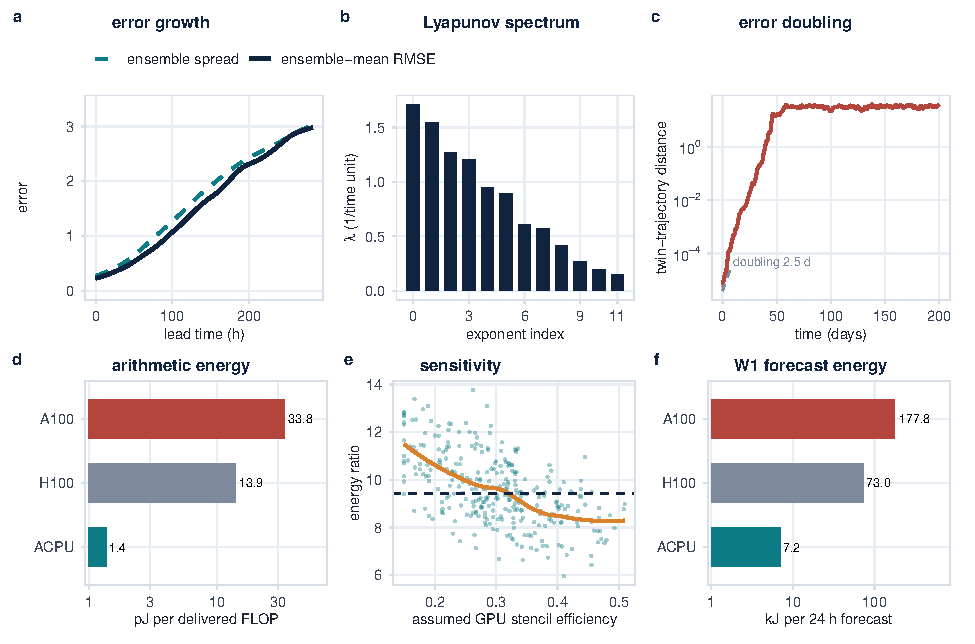
\includegraphics[width=\linewidth]{fig01_requirements}
\caption{Why atmospheric computation needs a different machine. (a) Ensemble-mean RMSE and
ensemble spread against lead time for the Lorenz--96 experiment; the spread tracks the error,
which is the property the precision governor exploits. (b) Leading Lyapunov exponents of the
Lorenz--96 attractor (per model time unit; one unit $\approx$ 5 days). (c) Twin-trajectory
distance on a log scale, giving a doubling time of \ACDoubling\ days. (d) Arithmetic intensity of
each kernel measured against HBM. (e) Dependence of the energy ratio on the assumed GPU stencil
efficiency (300 Monte-Carlo samples). (f) Energy per 24 h forecast for \ac{1}, an H100 and an A100.}
\label{fig:req}
\end{figure}
